\documentclass[conference]{IEEEtran}
% \documentclass[11pt,a4paper]{article}

\usepackage[utf8]{inputenc} % for utf8 encoded documents
\usepackage{mathrsfs,amsmath} % for \mathscr
\usepackage{enumitem} % for \setlist
\usepackage{indentfirst} % indent first paragraph
\usepackage{graphicx} % to include images
\usepackage{listings} % for \lstlisting and \lstinputlisting
\usepackage{comment} % for \comment and \endcomment
\usepackage{amsfonts} % for \mathbb
\usepackage{float} % for H placement specifier
\usepackage{hyperref} % for hyperlinks
\usepackage{cleveref} % for clever reference prefixes
\usepackage{caption} % for captions
\graphicspath{ {./results/} } % for images
\usepackage[section]{placeins} % for \FloatBarrier

\newenvironment{mathenum}[1][]{
\enumerate[#1]\mtmathitem}{$\endlist} 

\title {Network Security Term Project Report}
\author{Taha Adeel Mohammed  {\small CS20BTECH11052}, Shambhu Kavir {\small CS20BTECH11045}  }


\begin{document}

\maketitle

\section{Problem Statement}
\noindent
\textbf{Title:} Understanding and mitigating HTTP Request Smuggling attacks \hbadness=10000 \\

\noindent
\textbf{Description:} HTTP Request Smuggling (HRS) attack is a discovered vulnerability of HTTP where some header fields of HTTP header are exploited to smuggle the request. This vulnerability was exploited in 2005 itself but since then there are many ways and methodologies that are also explored which can launch this attack in numerous ways. Due to the significant amount of research done in this field, there are labs and repositories available to do hands-on practice. As part of the project, students are expected to understand, perform HSR attack practically, detecting it and deploying one mitigation technique. \hbadness=10000 \\

\noindent
\textbf{Steps to be performed:-}
\begin{enumerate}
	\item Understanding of HTTP Web Smuggling attack.
	\item Using existing labs/techniques to carry out attacks in a sandbox environment.
	\item Simulating the attack and check vulnerability of servers supporting HTTP 1.1 and HTTP 1.2. You should able to answer the following questions:-
	\begin{enumerate}
		\item How do you exploit HTTP 1.1 server with HRS?
		\item Are you able to exploit HTTP 1.2  server with HRS?
		\item Do you need a different payload/technique for both HTTP 1.1 and HTTP 1.2?
	\end{enumerate}
	\item Deploy mitigation techniques (your own proposed or from the existing solutions) to HRS.
\end{enumerate}

\noindent
\textbf{Deliverables:-}
\begin{enumerate}
	\item Code/tools/commands used to simulate/emulate HRS.
	\item Demonstration of attacks both in HTTP 1.1 and HTTP 1.2
	\item Demonstration of mitigation techniques
	\item Detailed report with methodology, observations, discussion and results.
	\item To check the impact of HRS on HTTP/3. To find possible vectors of HRS in HTTP/3 or to list down factors that secure it against HRS.
\end{enumerate}

\section{Project description}
\subsection*{Basics of HTTP Request Smuggling}
Majority of the web applications existing today employ HTTP servers between the users and the application logic. The requests from the user are sent to a front-end/reverse proxy(also called load balancer) which then forwards the request to the backend server. The backend server processes the request and sends the response back to the reverse proxy which then forwards the response to the user. \\

For this purpose, it is necessary for the front-end and backend to establish and adhere to certain rules while processing requests, failing which attackers might send ambiguous requests that get interpreted differently by the front-end and backend. This is called HTTP Request Smuggling. \\

The HTTP specification provides two different ways to specify the way in which the body of a request is to be interpreted. The first is the \textbf{Content-Length header}, which is used to specify the length of the body in bytes. The second is the \textbf{Transfer-Encoding header}, which is used to specify the type of encoding used to transmit the body. \\

As there are two different ways of specifying the length of the the requests, it is possible for a request to use both methods at once, resulting in ambiguity. Attackers take advantage of this ambiguity to send requests that are interpreted differently by the front-end and backend. \\

\begin{figure}[h]
	\centering
	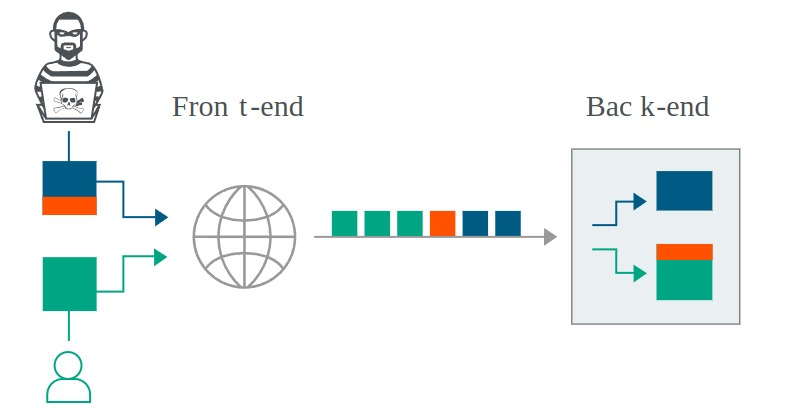
\includegraphics[width=0.45\textwidth]{results/HRS intro.jpeg}
	\caption{HTTP Request Smuggling (From \cite{lab2})}
	\label{fig:smuggling}
\end{figure}

The HTTP specification attempts to avoid this problem, by stating that when both headers are present, the Transfer Encoding should be enforced. However, this solution fails when there are multiple servers in the request chain, and one of the servers does not support Transfer-Encoding header or they can be manipulated to avoid processing the header. This leads to disagreements between the front-end and backend servers resulting in vulnerabilities. 

\subsection*{Exploiting HRS vulnerabilities in HTTP 1.1}
Exploiting HRS vulnerabilities involves having both TE and CL headers in one request such that the front-end processes one of the headers and the backend processes the other. There are three such ways to do this:
\begin{enumerate}
	\item \textbf{CL.TE} - The front-end processes the Content-Length header and the backend processes the Transfer-Encoding header. This is the most common type of HRS vulnerability. \\
	\begin{verbatim}
		POST / HTTP/1.1
		Host: vulnerable-website.com
		Content-Length: 13
		Transfer-Encoding: chunked
		
		0

		SMUGGLED
	\end{verbatim}
Here, the front end processes CL and the backend processes TE. The front-end will read the first 13 bytes of the body and then stop reading as it has reached the end of the body. The backend server processes TE and treats the request body as chunked encoding. The first chunk is processed and treated to be of 0 length. The remaining bytes, i.e. SMUGGLED are treated as the new request.  \\
	


	\item \textbf{TE.CL} - The front-end processes the Transfer-Encoding header and the backend processes the Content-Length header. \\
	\begin{verbatim}
		POST / HTTP/1.1
Host: vulnerable-website.com
Content-Length: 3
Transfer-Encoding: chunked

6
ATTACK
0
	\end{verbatim}
Here, the front end processes TE and the backend processes CL. The front-end will read the first chunk of 6 bytes and then stop reading as it has reached the end of the body. The backend server processes CL and treats the request body as 3 bytes long. The first 3 bytes, i.e. uptill the start of the word ATTACK are processed while the rest is treated as the start of a new request.  \\
	\item \textbf{TE.TE} - In this case, both the front-end and backend support the TE but one of them is manipulated and prevented from processing it.
	\begin{verbatim}
		Transfer-Encoding: xchunked

Transfer-Encoding : chunked

Transfer-Encoding: chunked
Transfer-Encoding: x

	\end{verbatim}
	In this example, one of either backend or front-end is manipulated into not processing one of the headers by obscuring it, while the request is smuggled in the other using the second header. \\
\end{enumerate}

\subsection*{HTTP 2 and its vulnerabilities}
HTTP 1.1 is a text-based protocol, wherein the requests are parsed using string operations. This gives room for plenty of ambiguity, which is exploited by attackers to smuggle requests. On the other hand, HTTP 2 is a binary protocol, which means that the requests are parsed using binary operations. \\

In HTTP 1.1 the length of the message request body is denoted by the TE or CL. However, in HTTP 2, the length of the message is denoted by the length of the frame. This makes it very difficult to smuggle requests using the same techniques as HTTP 1.1. \\

HSR attacks in HTTP 2 is done via a process called downgrading. In this process, the reverse proxy interacts with the client in HTTP 2 but forwards the requests to the backend in HTTP 1.1. This transition in protocol makes it possible to smuggle requests. \\

In HTTP 2, the frontend generally uses HTTP 2's built in length. However, the backend which recieves the downgraded request and has no access to this built in length. Therefore, it has to pick between one of TE and CL. This gives rise to two kinds of vulnerabilities
\begin{enumerate}
	\item \textbf{H2.CL} - Consider the following HTTP 2 request
	\begin{verbatim}
		:method	POST
:path	/n
:authority	www.netflix.com
content-length	4
abcdGET /n HTTP/1.1
Host: 02.rs?x.netflix.com
Foo: bar
	\end{verbatim}

After downgrading, it looks like
\begin{verbatim}
	POST /n HTTP/1.1
Host: www.netflix.com
Content-Length: 4

abcdGET /n HTTP/1.1
Host: 02.rs?x.netflix.com
Foo: bar
\end{verbatim}
The backend which uses CL, stops processing the request body early, due to the incorrect length, and treats the rest of the request as a new request. This is the H2.CL vulnerability. \\

\item \textbf{H2.TE} - Consider the following HTTP 2 request
\begin{verbatim}
	:method	POST
:path	/identitfy/XUI
:authority	id.b2b.oath.com
transfer-encoding	chunked
0

GET /oops HTTP/1.1
Host: psres.net
Content-Length: 10

x=
\end{verbatim}
After downgrading, it looks like
\begin{verbatim}
	POST /identity/XUI HTTP/1.1
Host: id.b2b.oath.com
Content-Length: 66
Transfer-Encoding: chunked

0

GET /oops HTTP/1.1
Host: psres.net
Content-Length: 10

x=
\end{verbatim}
When the backend uses TE and assumes the data is in chunked bytes, it sees the first chunk of 0 length and stops processing the request body. The rest of the request is treated as a new request. This is the H2.TE vulnerability. \\

\subsubsection*{h2c Smuggling}
h2c or HTTP/2 Cleartext smuggling is another type of HTTP request smuggling targeting web applications using HTTP/2 protocol in cleartext. In HTTP/2, each message  is split into smaller frames and transmitted which are then reassembled at the reciever. However, the way the reverse proxy and backend handle these frames can vary, giving room for exploitable vulnerabilities. \\
In this case, the attacker sends a request that appears to contain multiple HTTP/2 frames, but it is actually constructed in such a way that the different components interpret them differently. As a result its possible that one of frontend and backend might interpret the request as a single frame, while the other might interpret it as multiple frames. This can be exploited to smuggle requests. \\
\end{enumerate}

\subsection*{Mitigation Techniques}
\begin{itemize}
	\item Prioritizing TE over CL headers - In case the request contains both the headers, TE should be enforced over CL. This is because, TE can cover both static and dynamic requests, while CL can only cover static requests.
	\item Securing logged HTTP Traffic - The HTTP logs should be secured and be accessible only to authorized personnel. This is because, the logs can be used by attackers to find out the vulnerabilities in the system and exploit them, thus preventing attackers from accessing unintended parts of HTTP requests.
	\item Rejecting requests with double headers - Requests containing TE.CL, CL.TE and TE.TE headers should be rejected with a 400 Bad Request response, so as to avoid ambiguity between the front-end and the backend in processing the request.
	\item Using Vulnerability Scanner -  Vulnerability scanners can be employed to detect poorly configured HTTP requests. Periodic testing should be enforced in web applications to reduce the risk of attacks.
	\item Enforcing HTTP 2 - Using HTTP 2 both in the front end and the back end can help prevent HSR attacks to a huge extent as it does not allow ambiguity in parsing requests.
\end{itemize}

\subsection*{HTTP 3}
HTTP/3 is a relatively new protocol that is still being developed. It is based on QUIC, which is a transport layer protocol, and is designed to be secure, low-latency and multiplexed. Although it is possible that new vulnerabilities may be introduced, it has been designed with security in mind and is intended to prevent commmon HRS attacks which work on HTTP 1 and 2, among other improvements. \\
These include
\begin{itemize}
	\item HTTP/3 separates individual requests and responses into separate streams, each of which is transmitted separately of each other. THis prevents the ambiguity in parsing requests and responses which is present in HTTP 1 and 2.
	\item HTTP/3 employs a new framing mechanism called QUIC Datagram, which is a small, self contained packet that carries a single HTTP/3 frame, each of which is carried independent of the others. This makes it difficult for the attackers to intercept or modify the data in transit.
	\item HTTP/3 uses explicit stream multiplexing, meaning each individual request/response is mapped to a unique stream identifier that is explicitly specified in the protocol. This ensures that each request and response is unambiguously associated with a particular stream, removing any confusion alleviating the room for misinterpretation between the frontend and backend.
\end{itemize}


\section{Project Implementation and Results}
To demonstrate the working of HTTP Smuggling Request attacks, and the ways to detect and exploit the vulnerability, we used the labs provided by portswigger which provide us with servers and proxies in between such that they are vulnerable to our HRS attacks. We then use the BURP suite to send requests to these servers in such a manner as to exploit these vulnerabilities and demonstrate the attacks. Below are the major HRS demonstrations and their results:

\subsection*{Basic CL.TE HRS attack}
Here, the front-end server uses the Content-Length header and the back-end server uses the Transfer-Encoding header. Figure \ref*{fig:ce.te} shows the request and response from the server on sending the shown request twice. As we can see, the first time the server responds as expected, but for the second request, we get the response "Invalid method GPOST" because the smuggled G from the last request was appended to the POST of the second request.

\begin{figure}[htbp]
	\centering
	\begin{minipage}[c]{0.45\linewidth}
	  \centering
	  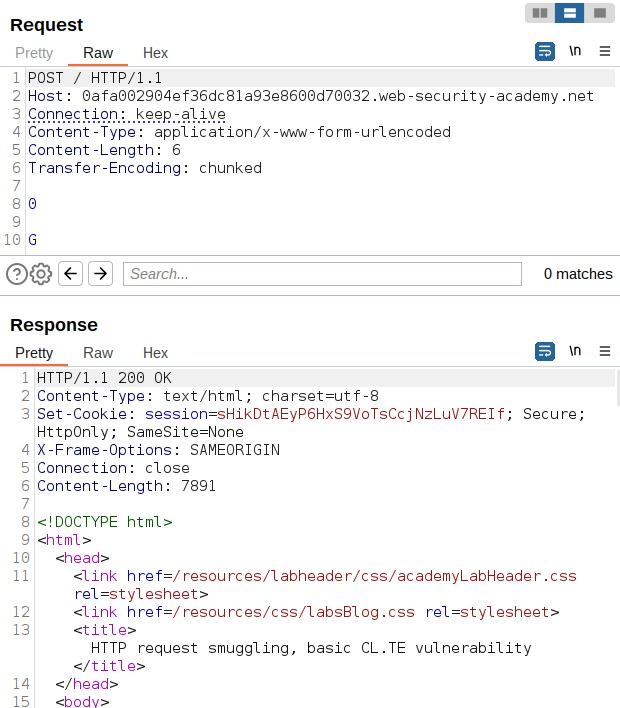
\includegraphics[width=\linewidth]{results/CL.TE_req1_OK_response.jpeg}
	  \caption*{Req-1: Expected response}
	  \label{fig:ce.te_req1_ok}
	\end{minipage}
	\hfill
	\begin{minipage}[c]{0.45\linewidth}
	  \centering
	  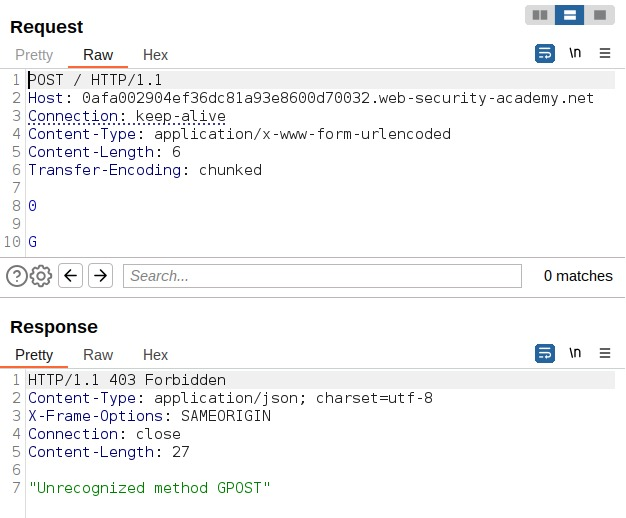
\includegraphics[width=\linewidth]{results/CL.TE_req2_GPOST_invalid.jpeg}
	  \captionsetup{justification=centering}
	  \caption*{Req-2: Smuggling \\ successful}
	  \label{fig:ce.te_req2_gpost}
	\end{minipage}
  
	\caption{CE.TE HRS attack}
	\label{fig:ce.te}
  \end{figure}

\subsection*{Basic TE.CL HRS attack}
Here, the front-end server uses the Transfer-Encoding header and the back-end uses the Content-Length header. Similar to the previous attack, in Figure \ref*{fig:te.cl}, we smuggle 'G' to the backend, causing the server to respond with "Invalid method GPOST" for the second request.

\begin{figure}[htbp]
	\centering
	\begin{minipage}[c]{0.45\linewidth}
	  \centering
	  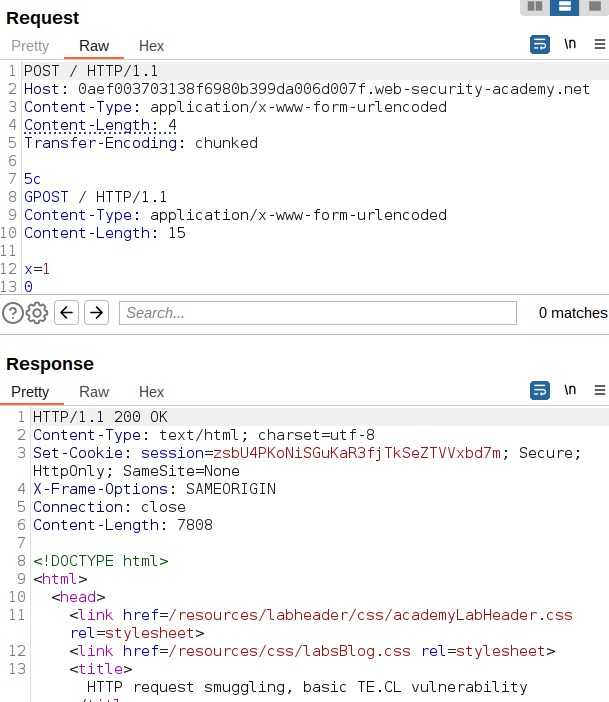
\includegraphics[width=\linewidth]{results/TE.CL_req1_OK_response.jpeg}
	  \caption*{Req-1: Expected response}
	  \label{fig:te.cl_req1_ok}
	\end{minipage}
	\hfill
	\begin{minipage}[c]{0.45\linewidth}
	  \centering
	  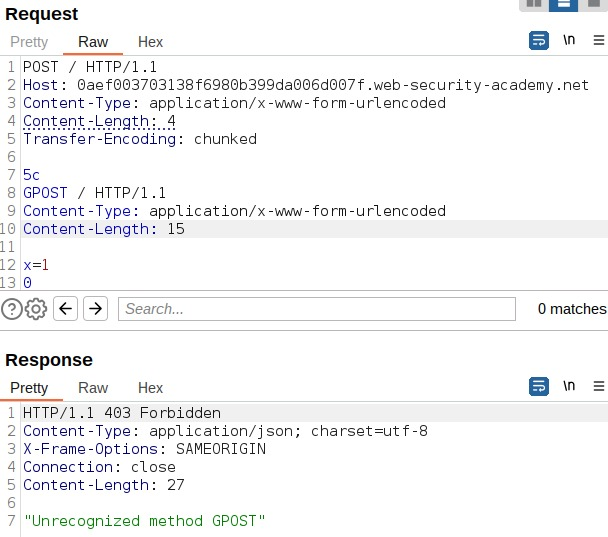
\includegraphics[width=\linewidth]{results/TE.CL_req2_GPOST_invalid.jpeg}
	  \captionsetup{justification=centering}
	  \caption*{Req-2: Smuggling \\ successful}
	  \label{fig:te.cl_req2_gpost}
	\end{minipage}
  
	\caption{TE.CL HRS attack}
	\label{fig:te.cl}
\end{figure}

\subsection*{Basic TE.TE HRS attack}
Here, the front-end and back-end servers both support the Transfer-Encoding header, but one of the servers can be induced not to process it by obfuscating the header in some way. One example run can be seen in Figure \ref*{fig:te.te}.

\begin{figure}[htbp]
	\centering
	\begin{minipage}[c]{0.45\linewidth}
	  \centering
	  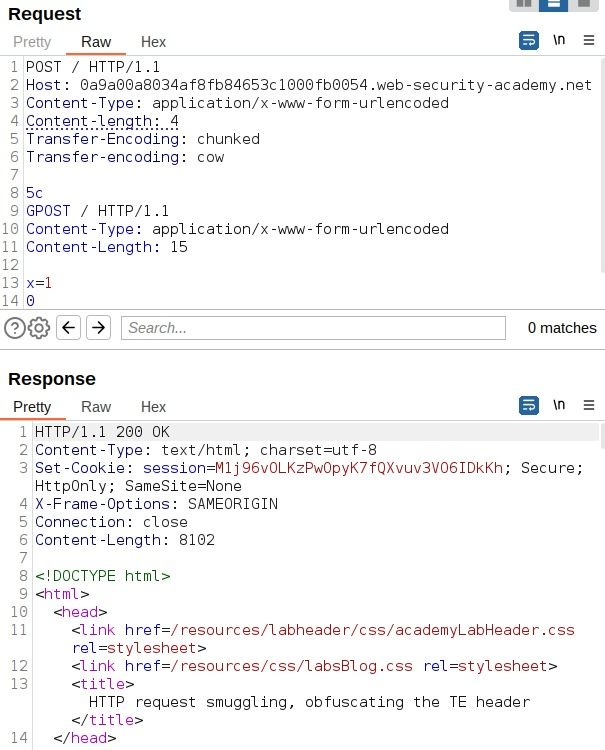
\includegraphics[width=\linewidth]{results/TE.TE_req1_OK_response.jpeg}
	  \caption*{Req-1: Expected response}
	  \label{fig:te.te_req1_ok}
	\end{minipage}
	\hfill
	\begin{minipage}[c]{0.45\linewidth}
	  \centering
	  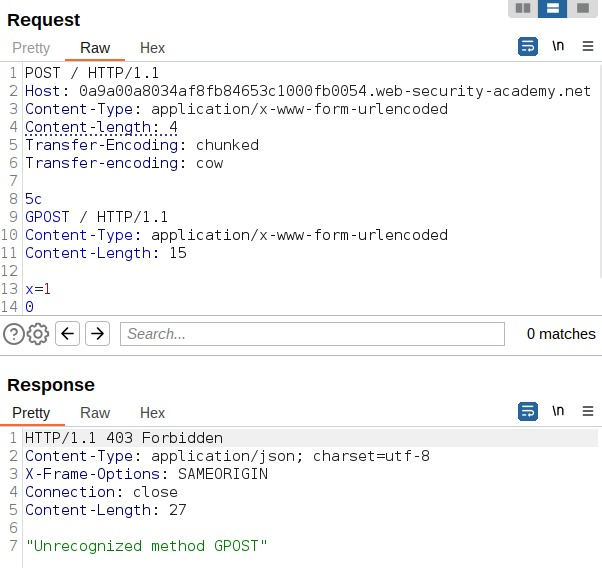
\includegraphics[width=\linewidth]{results/TE.TE_req2_GPOST_invalid.jpeg}
	  \captionsetup{justification=centering}
	  \caption*{Req-2: Smuggling \\ successful}
	  \label{fig:te.te_req2_gpost}
	\end{minipage}
  
	\caption{TE.TE HRS attack}
	\label{fig:te.te}
\end{figure}

\subsection*{Detecting CL.TE using differential response}
Over here, we send a request in such a manner such that the server will respond with a "404 not found" response if it has CL.TE vulnerability, and responds normally if it doesn't, as in Figure \ref*{fig:ce.te.detection}. Note that the output result images henceforth are majorly for when we send the request the second time, as thats when the smuggled request is processed.

\begin{figure}[htbp]
	\centering
	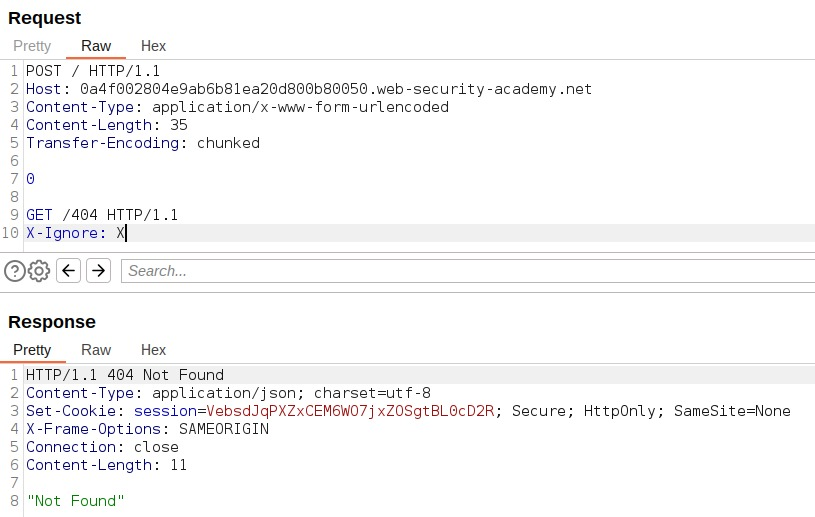
\includegraphics[width=0.4\textwidth]{results/Detecting_CL.TE.jpeg}
	\caption{Detecting CL.TE using differential response}
	\label{fig:ce.te.detection}
\end{figure}

\subsection*{Detecting TE.CL using differential response}
Similarly, Figure \ref*{fig:te.cl.detection} shows how TE.CL vulnerability can be detected using differential responses.

\begin{figure}[htbp]
	\centering
	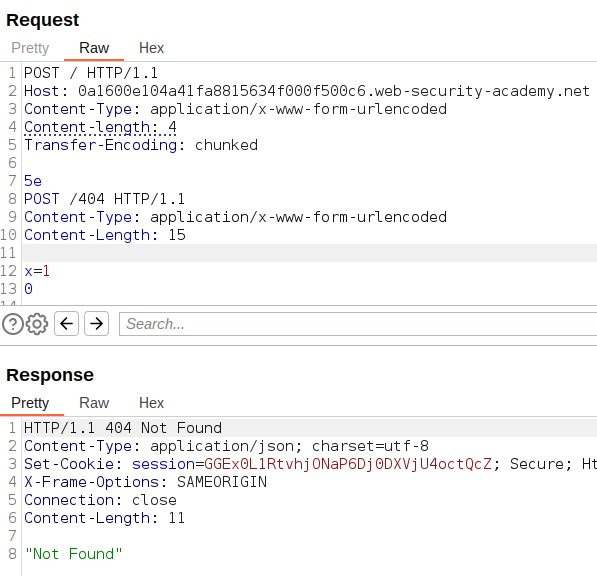
\includegraphics[width=0.4\textwidth]{results/Detecting_TE.CL.jpeg}
	\caption{Detecting TE.CL using differential response}
	\label{fig:te.cl.detection}
\end{figure}

\subsection*{Using HRS to bypass front-end security controls}
Some applications have the front-end web server implement some security controls to allow individual requests to be processed, and then forward the allowed requests to the backend. We can bypass these checks by smuggling in the illegal request to the backend, and gaining unauthorized perks. For example, in Figure \ref*{fig:bypass}, we smuggle in a request to delete the user carlos on the path "\textbackslash admin", which is normally inaccessible to remote users. 

\begin{figure}[htbp]
	\centering
  
	\begin{minipage}{\linewidth}
	  \centering
	  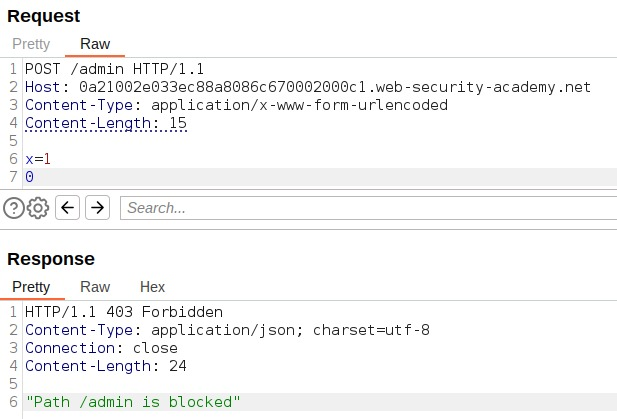
\includegraphics[width=0.6\linewidth]{results/Bypass_frontend_req0_admin_blocked.jpeg}
	  \captionsetup{justification=centering}
	  \caption*{Normal requests to \textbackslash admin blocked}
	  \label{fig:bypass_req0}
	\end{minipage}
  
	\vspace{\baselineskip} % Add vertical spacing between the first and second row of images
  
	\begin{minipage}[t]{0.45\linewidth}
	  \centering
	  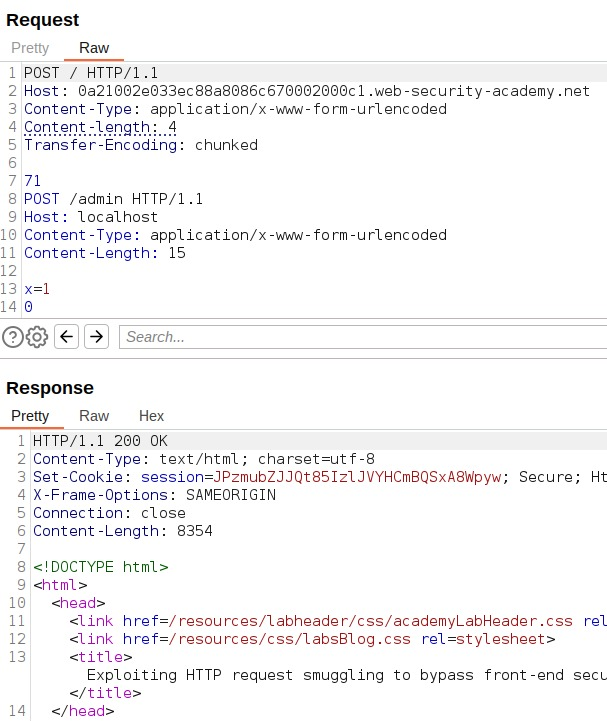
\includegraphics[width=\linewidth]{results/Bypass_frontend_req1_OK_response.jpeg}
	  \caption*{Smuggling request to admin}
	  \label{fig:bypass_req1}
	\end{minipage}
	\hfill
	\begin{minipage}[t]{0.45\linewidth}
	  \centering
	  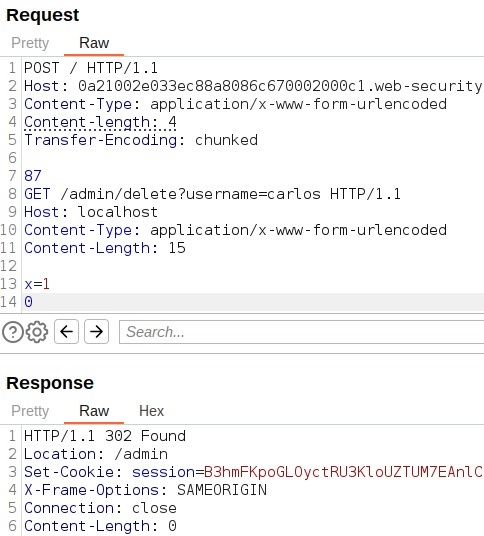
\includegraphics[width=\linewidth]{results/Bypass_frontend_req2_deleting_carlos_successful.jpeg}
	  \captionsetup{justification=centering}
	  \caption*{Carlos deleted successfully}
	  \label{fig:bypass_req2}
	\end{minipage}
  
	\caption{Using HRS to bypass front-end security controls}
	\label{fig:bypass}
\end{figure}

\subsection*{Revealing frontend request rewriting}
Sometimes the front-end server might add some extra headers to the request before forwarding it to the backend, and these headers might interfere with our HRS attacks. This request rewriting can be revealed by haveing our smuggled requests content-length header be much larger than the its actual body, so that in the servers response, the next message (rewritten) is considered a part of the smuggled request and sent back to the attacker. In Figure \ref*{fig:rewriting}, we can see that the front-end adds an X-IP header to our request, which we managed to reveal.

\begin{figure}[htbp]
	\centering
	\begin{minipage}[c]{0.45\linewidth}
		\centering
		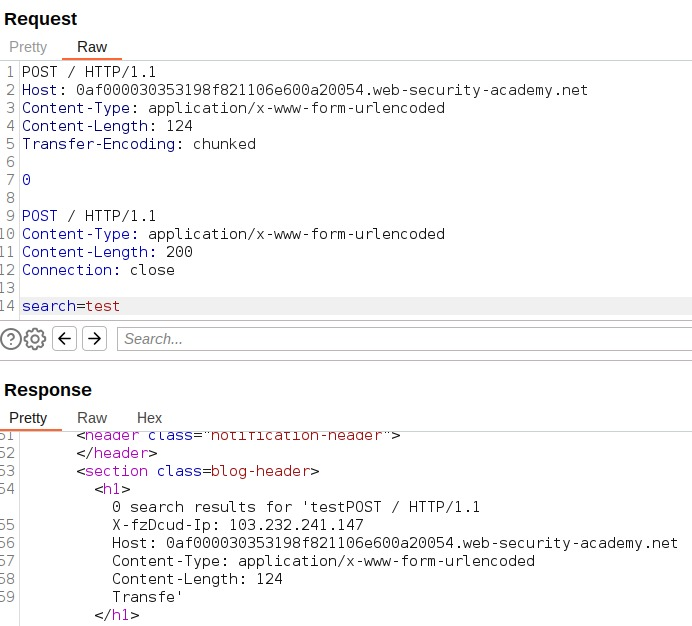
\includegraphics[width=\linewidth]{results/Frontend_request_rewriting_req1_revealing.jpeg}
		\captionsetup{justification=centering}
		\caption*{Revealing the rewritten request}
		\label{fig:rewriting_req1}
	  \end{minipage}
	  \hfill
	  \begin{minipage}[c]{0.45\linewidth}
		\centering
		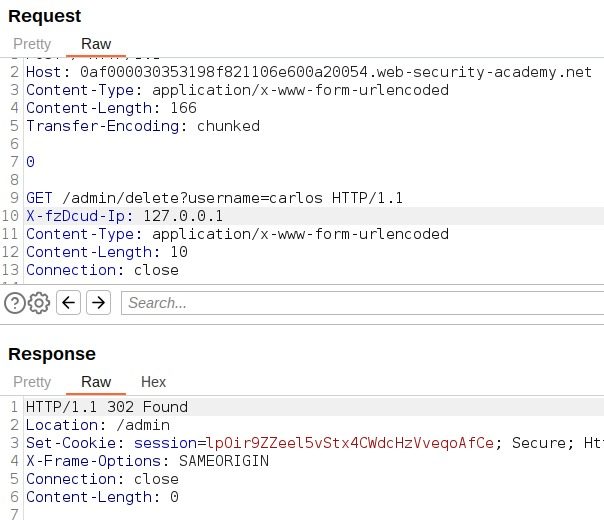
\includegraphics[width=\linewidth]{results/Frontend_request_rewriting_req2_exploiting.jpeg}
		\captionsetup{justification=centering}
		\caption*{Exploiting the revealed request to delete Carlos}
		\label{fig:rewriting_req2}
	  \end{minipage}
	
	  \caption{Revealing frontend request rewriting}
	  \label{fig:rewriting}
\end{figure}

In a similar manner, it is also possible to reveal other users data/requests, compromising their privacy.

\subsection*{Performing XSS injection}
By exploiting a reflected XSS vulnerability in an application, an attacker can inject a malicious payload into a request header. This payload will be reflected back in the response received by the next user who visits the page. Figure \ref*{fig:xss} illustrates this scenario, where the XSS payload is in the User-Agent header. Once the payload is reflected in the response, the attacker can utilize the reflected XSS vulnerability to execute malicious actions on the user's system.

\begin{figure}[htbp]
	\centering
	\begin{minipage}[c]{0.45\linewidth}
		\centering
		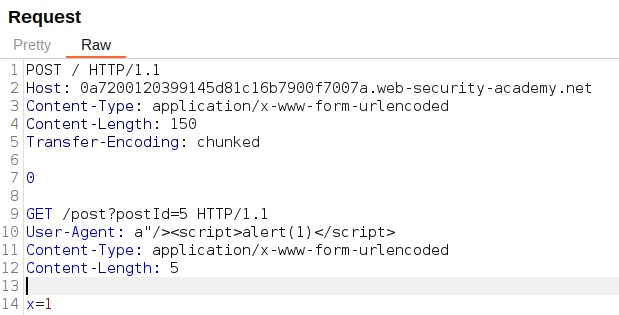
\includegraphics[width=\linewidth]{results/XSS_injection_code.jpeg}
		\captionsetup{justification=centering}
		\caption*{XSS injection smuggling request}
		\label{fig:xss_req}
	  \end{minipage}
	  \hfill
	  \begin{minipage}[c]{0.45\linewidth}
		\centering
		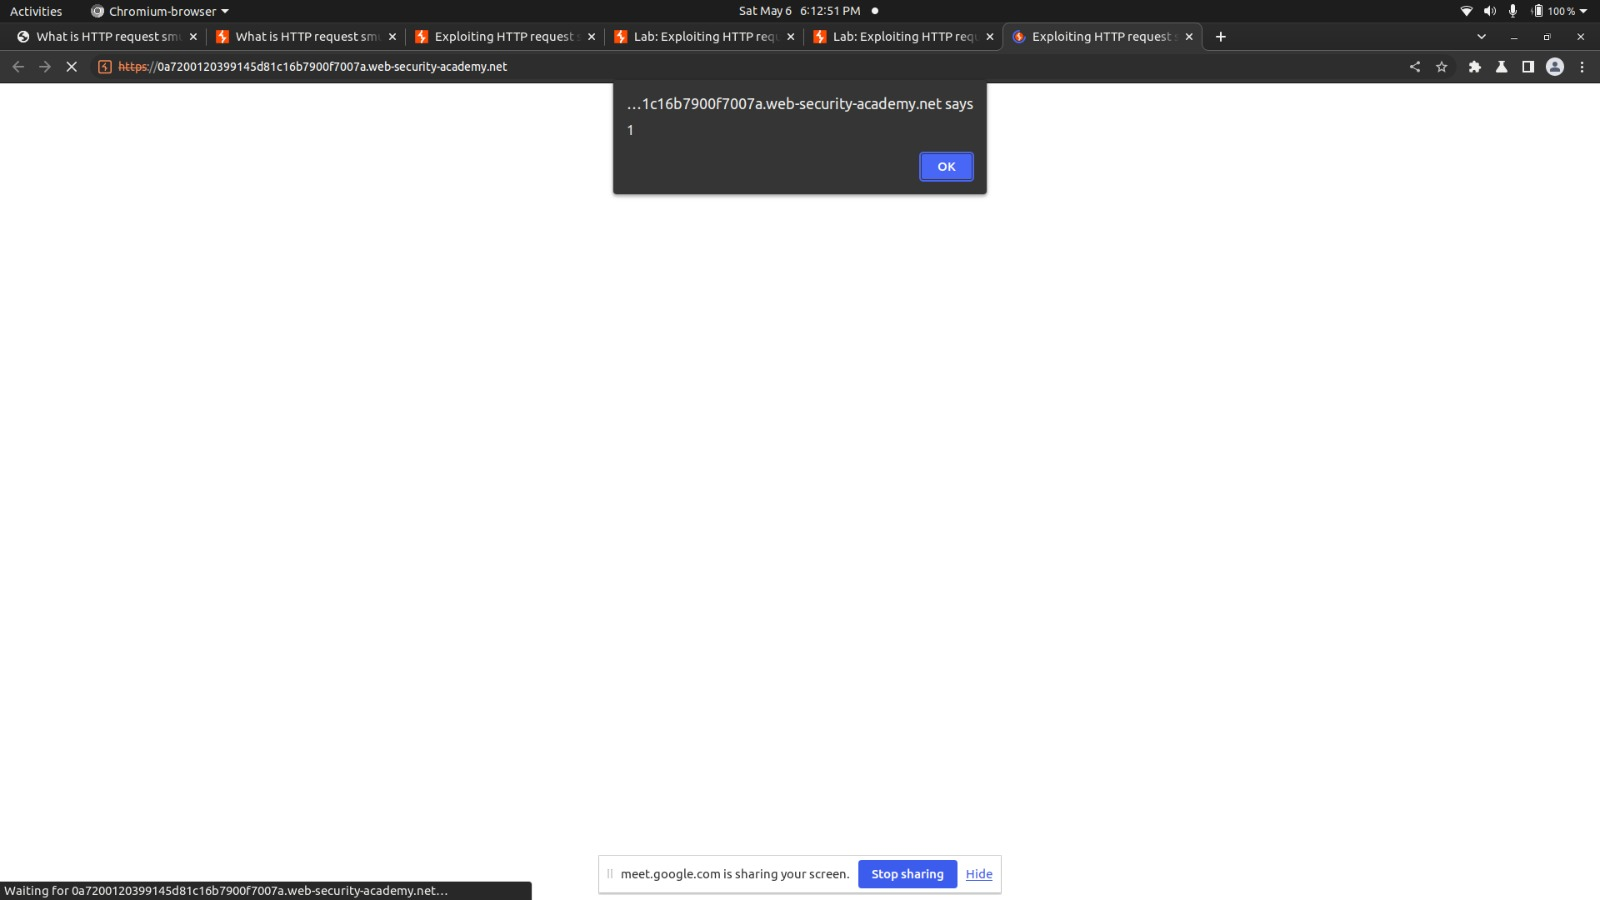
\includegraphics[width=\linewidth]{results/XSS_injection_result.jpeg}
		\captionsetup{justification=centering}
		\caption*{Next user receiving the XSS payload}
		\label{fig:xss_response}
	  \end{minipage}
	
	  \caption{Performing XSS injection}
	  \label{fig:xss}
\end{figure}

\vspace*{2mm}
\par{ \noindent
	HRS attacks can also be used to turn an on-site redirect into an open redirect, potentially redirecting the users who request some harmless script to a script from the attacker that can take control of their entire system. We can also perform web-cache poisoning such that all user requests to a particular front-end web server are affected, instead of just the next one in the queue.   
}


\section{Simulation/Experimentation Setup}
To demonstrate the mitigation techniques for HRS attacks in a sandbox environment, we attempted to set up a reverse proxy in a docker environment using nginx, as well as client and server side code using socket programming and flask respectively to simulate the attacks. These files can be found in the './simulation' folder, and the instructions to run them can be found in its readme.  However, we were unable to demonstrate our own mitigation techniques as nginx by default rejects any requests with both the Content-Length and Transfer-Encoding headers, hence preventing any HRS attacks. We were unable to find a way to disable this behaviour, and as the http request smuggling attacks are already mitigated in nginx, which is one of the most popular reverse proxies, we just note that as our mitigation technique. I.e, use the latest standard tools and techniques for your applications, as they would most likely be patched agaisnt most security vulnerabilities.


\section{Conclusion}
\begin{itemize}
    \item HTTP request is a serious vulnerability in the HTTP protocol that can be exploited to launch on web servers.
    \item Through hands on practice and research, we have gained deep understanding of how HRS works and different techniques that we can use to exploit it.
    \item It is important for web developers and security professionals to be aware of this vulnerability and take measures to prevent it.
\end{itemize}

\section{Contirbutions}
\begin{enumerate}
    \item Taha:- Simulating attacks in HTTP 1.1 in port swigger labs, HTTP smuggling vulnerability detection methods, ways attacks can be carried out to exploit the vulnerability, researching mitigation techniques, setting up reverse proxy in sandbox environment for attempting mitigation techniques, report writing, presentation.
    \item Shambhu:- Simulating detection methods and attacks in HTTP 1.1 and HTTP 2 in a docker environment, including downgrading and h2c, methods to mitigate attacks in HTTP 2, setting up reverse proxy for attempting mitigation techniques, exploring improvements in HTTP 3, report writing, presentation.
\end{enumerate}

\begin{thebibliography}{9}

\bibitem{reference1} https://www.hindawi.com/journals/scn/2022/3121177/
\bibitem{reference2} https://ieeexplore.ieee.org/stamp/stamp.jsp?tp=\&arnumber=9626191
\bibitem{reference3} https://i.blackhat.com/USA-20/Wednesday/us-20-Klein-HTTP-Request-Smuggling-In-2020-New-Variants-New-Defenses-And-New-Challenges-wp.pdf
\bibitem{reference4} https://bishopfox.com/blog/h2c-smuggling-request 
\bibitem{lab1} https://gosecure.github.io/request-smuggling-workshop/\#0
\bibitem{lab2} https://portswigger.net/web-security/request-smuggling
\bibitem{lab3} https://github.com/BishopFox/h2csmuggler

\end{thebibliography}



\subsection*{Anti-Plagiarism Statement}
I certify that this assignment/report is my own work, based on my personal study and/or research and that I have acknowledged all material and sources used in its preparation, whether they be books, articles, reports, lecture notes, and any other kind of document, electronic or personal communication. I also certify that this assignment/report has not previously been submitted for assessment in any other course, except where specific permission has been granted from all course instructors involved, or at any other time in this course, and that I have not copied in part or whole or otherwise plagiarised the work of other students and/or persons. I pledge to uphold the principles of honesty and responsibility at CSE@IITH. In addition, I understand my responsibility to report honour violations by other students if I become aware of it.\\

\noindent
Name: Taha Adeel Mohammed and Shambhu Kavir \\
Date: \today \\
Signature: T.A.M. and S.K.


\end{document}